\documentclass[12pt]{report}
\usepackage[utf8]{inputenc}
\usepackage[a4paper,width=160mm,top=25mm,bottom=25mm]{geometry}
%---------------------------------
\usepackage{graphicx}
\usepackage{subcaption}
\usepackage[font=footnotesize]{caption}
\captionsetup{justification=centering, labelfont=sc, labelsep=endash}
\graphicspath{ {images/} }
%---------------------------------
\usepackage{acro}
\DeclareAcronym{who}{
  short = WHO ,
  long  = World Health Organization ,
  class = abbrev
}

\DeclareAcronym{ltbi}{
  short = LTBI ,
  long  = Latent Tuberculosis Infection ,
  class = abbrev
}

\DeclareAcronym{tb}{
  short = TB ,
  long  = Tuberculosis ,
  class = abbrev
}

\DeclareAcronym{hiv}{
  short = HIV ,
  long  = Human Immunodeficiency Virus ,
  class = abbrev
}

\DeclareAcronym{ct}{
  short = CT ,
  long  = Computed Tomography ,
  class = abbrev
}

\DeclareAcronym{bk}{
  short = BK ,
  long  = Bacillus Koch ,
  class = abbrev
}

\DeclareAcronym{3d}{
 short  = 3D,
 long   = 3 Dimensions,
 class  = abbrev
}

\DeclareAcronym{nifti}{
 short  = Nifti,
 long   = Neuroimaging Informatics Technology Initiative,
 class  = abbrev
}

\DeclareAcronym{minc}{
 short  = Minc,
 long   = Medical Imaging NetCDF,
 class  = abbrev
}

\DeclareAcronym{dicom}{
 short  = Dicom,
 long   = Digital Imaging and Communications in Medicine,
 class  = abbrev
}

\DeclareAcronym{jpeg}{
 short  = JPEG,
 long   = Joint Photographic Experts Group,
 class  = abbrev
}

\DeclareAcronym{rle}{
 short  = RLE,
 long   = Run-Length Encoding,
 class  = abbrev
}

\DeclareAcronym{mpeg}{
 short  = MPEG,
 long   = Moving Picture Experts Group,
 class  = abbrev
}


%---------------------------------

%---------------------------------
\usepackage{fancyhdr}
\pagestyle{fancy}
\fancyhead{}
% \fancyhead[RO,LE]{Thesis Title}
\fancyfoot{}
% \fancyfoot[LE,RO]{\thepage}
% \fancyfoot[LO,CE]{Chapter \thechapter}
% \renewcommand{\headrulewidth}{0.4pt}
% \renewcommand{\footrulewidth}{0.4pt}
%---------------------------------

%--------------------------------
\begin{document}
 \begin{titlepage}
   \begin{center}
       \vspace*{1cm}
 
       \large \textbf{Automatic Tuberculosis Severity Scoring Using Machine Learning Techniques}
        \normalsize
       \vspace{0.5cm}
 
       \vspace{1.5cm}
 
       \textbf{Author : Noreddine BELHADJ CHEIKH}\\
       \textbf{Supervised by : Abdelkader HAMADI }
        \vspace{0.5cm}
 
       \vspace{1.5cm}
 
       A thesis submitted for the Master's degree 
       in Engineering of Information Systems
       \vspace{0.5cm}
 
       \vspace{1.5cm}
       
       
\includegraphics[width=0.4\textwidth]{university.png}\\
       \vfill
       Faculty of Exact Science and Informatics\\
       University Of Mostaganem Abdelhamid Ibn Badis\\
       Algeria\\
       25 February, 2019
    
   \end{center}
\end{titlepage}
 

 %-------------------------------
\chapter*{Abstract}
Abstract goes here here

\tableofcontents
%-------------------------------
\chapter*{Introduction}
\addcontentsline{toc}{chapter}{Introduction}
\paragraph{}
In recent decades, medical imaging has become indispensable in the diagnosis and therapy of diseases. With the enhancement of medical imaging databases, new methods are required to better handle this huge volume of data. However, because of the large variations and complexity of medical imaging data, it is generally difficult to deduce analytical solutions or simple methods to describe and represent objects such as lesions and anatomies in data. Therefore, medical imaging tasks require learning from the examples, and this is one of the key interests of the machine learning field.
\paragraph{}
Machine learning has become one of the main tools for medical image analysis. Machine learning techniques are solutions for developing tools to help physicians diagnose, predict, and prevent the risk of disease before it becomes too late in less time. Deep Learning is a new component in the field of machine learning that encompasses a wide range of network architectures designed to perform multiple tasks. The first use of neural networks for medical image analysis goes back more than twenty years, their use has increased by several orders of magnitude over the last five years. different, articles \cite{NNMEEX:1,NNMEEX:2,NNMEEX:3,NNMEEX:4,NNMEEX:5} have highlighted the application of deep learning to a wide range of medical image analysis tasks (segmentation, classification, detection, recording, image reconstruction, enhancement, etc.).
\paragraph{}
Tuberculosis is an infectious disease caused by a bacterium called Bacillus mycobacterium tuberculosis \cite{TBT:1}. In 2018, 10 million people fell ill with \ac{tb}, and 1. 6 million died from the disease \cite{TBT:1}. This disease remained one of the top ten leading causes of death in the world in 2018 \cite{TBT:1}. Tuberculosis attacks the lungs but can also affect other parts of the body \cite{TBT:2}. Accurate and rapid diagnosis is the key to controlling this disease, but traditional \ac{tb} tests produce inaccurate or time consumnig results to be definitive. Researchers have been interested in this disease, particularly in the context of the ImageCLEF 2018\cite{ImageCLEF:1} international challenge \cite{ImageCLEF:1} where two tasks have been reserved for it. Algorithms involving deep learning have been tested to diagnose the presence or absence of tuberculosis. The results obtained were interesting. Indeed, the algorithms have achieved an impressive accuracy rate up to 96\% \cite{NNMEEX:6,NNMEEX:7} a result that is better than the intervention of many radiologists.
\paragraph{}
The goal of our project is to automatically give score of \ac{tb} severity via \ac{ct} scan. One of the possible applications of this study is to accelerate the diagnosis of the disease from a radiology image without resorting to expensive medical tests. This work is part of the ImageCLEF2018  task of classifying types of \ac{tb}, which has shown more promising results. We explore in this paper the different work and different concepts that link with this problem. Starting by giving an overview of tuberculosis and its types in chapter 1. Then, discuss the relationship between artificial intelligence and medical images and give definition of some important parts of these fields in chapter 2. In chapter 3, the ImageCLEF Tasks are described and the related work of tuberculosis severity scoring is reviewed.
\chapter{Pulmonary Tuberculosis and its types}
\paragraph{}
Tuberculosis is a chronic infectious disease caused by a bacterium. called " Mycobacterium Tuberculosis" or Bacillus Koch (\ac{bk}). Its most current and most common form (85\% of cases) is pulmonary tuberculosis, but there are also extra-pulmonary forms such as bone tuberculosis, ganglion tuberculosis and renal tuberculosis.
\paragraph{}
Tuberculosis can develop rapidly after the first contact with the microbe, but it can also appear several years later.
\section{Latent \ac{tb} infection (\ac{ltbi})}
\paragraph{}
\ac{ltbi} is the presence of tubercle bacilli within the body without manifestation of the disease. \ac{ltbi} carriers are by definition non-contagious and pose no risk to those around them.
\section{Active tuberculosis}
\paragraph{}
Active tuberculosis is a condition in which the body’s immune system is unable to fight off or defend against the Mycobacterium tuberculosis bacterium. This inability causes an infection of the lungs, which is the most common presentation, or other parts of the body (tuberculosis is a multisystemic disease). Apart from the respiratory system, the organ systems most commonly affected include the gastrointestinal systemT, the musculoskeletal system, the lymphoreticular system, and the reproductive system, as well as the skin and the liver.
\paragraph{}
Globally, the best estimate is that 10.0 million people (range, 9.0–11.1 million) developed \ac{tb} disease in 2017: 5.8 million men, 3.2 million women and 1.0 million children \cite{TBT:3}. There were cases in all countries and age groups, but overall 90\% were adults (aged ≥15 years), 9\% were people living with \ac{hiv} (72\% in Africa) and two thirds were in eight countries: India (27\%), China (9\%), Indonesia (8\%), the Philippines (6\%), Pakistan (5\%), Nigeria (4\%), Bangladesh (4\%) and South Africa (3\%). These and 22 other countries in \ac{who}’s list of 30 high \ac{tb} burden countries accounted for 87\% of the world’s cases\cite{TBT:3}.4 Only 6\% of global cases were in the \ac{who} European Region (3\%) and \ac{who} Region of the Americas (3\%)\cite{TBT:3}. 
\chapter{Medical Imaging and Machine Learning}
\section{Medical imaging}
\paragraph{}
Medical imaging encompasses the technologies and processes of creating visual representations out of an anatomical volume in a form of images to be used for clinical diagnosis, medical intervention, and disease monitoring.
\subsection{Medical imaging technologies}
\paragraph{}
Common medical imaging technologies include ones which use electromagnetic radiations such as X-ray imaging and Computed Tomography (\acs{ct}) imaging, others use sound waves and magnetic field such as ultrasound an magnetic resonance imaging.
\paragraph{X-ray imaging}
this technology is the oldest and the most frequently used, it works on wavelengths and frequencies that can penetrate through the skin creating a visualization of the inner body. It used to detect skeletal system malfunctioning, cancer through mammography, and other diagnoses that involve the visualization of the inner body. This technique comes with risks associated with the use of X-ray radiation.
\paragraph{\acs{ct} imaging}
is a form of X-ray imaging that produces a \acs{3d} visualization of for diagnosis, providing greater quality and detailed imaging of the internal organs, bones, blood vessels, soft tissues within the body.
it also inherits the risk of X-ray imaging whereas the benefits exceed its risk where in many cases the use of \acs{ct} scans prevents the need for exploratory surgery.
\paragraph{Ultrasound imaging}
uses High-frequency sound waves that are transmitted from the probe to the body via the conducting gel, those waves then bounce back when they hit the different structures within the body and that is used to create an image for diagnosis.
This technology is considered the safes without any recorded side effects of its usage and is the most cost-effective. Due to its low risk, it is the first choice for pregnancy.
\paragraph{Magnetic resonance imaging}
uses a strong magnetic field and radio waves it enables an in-depth view of the inside of a joint or ligament to be seen, rather than just the outside as in the case of \acs{ct} scans and X-ray. It has risks associated with the use of a strong magnetic field where any kind of metal implant, artificial joint could be moved or heated up within the magnetic field.
\subsection{Medical imaging Archiving and Recording} 
\paragraph{}
due to the nature of a medical image, storing it is different from storing regular images. Medical image data set consists typically of one or more images representing the projection of an anatomical volume onto an image plane (projection or planar imaging), a series of images representing thin slices through a volume (tomographic or multislice two-dimensional imaging), a set of data from a volume (volume or three-dimensional imaging), or multiple acquisition of the same tomographic or volume image over time to produce a dynamic series of acquisitions (four-dimensional imaging).\cite{ME:1}
\paragraph{}
There exist several medical images file formats all of them sharing the goal of standardizing medical images storage and transmission. Major file formats widely used in medical imaging are Analyze, Neuroimaging Informatics Technology Initiative (Nifti), \acs{minc}, and Digital Imaging and Communications in Medicine (\acs{dicom}).
\paragraph{Analyze}
Analysis 7.5 was created in the late 1980s as a format used by the Analyze commercial software developed at the Mayo Clinic in Rochester, MN, USA. For more than a decade, the format was the standard for post-processing medical imaging. The big point of view of the Analyze format is that it was designed for multidimensional (volume) data. Indeed, it is possible to store 3D or 4D data in a file (the fourth dimension being typically the temporal information). An Analyze 7.5 volume includes two binary files: an image file with the extension .img which contains the raw voxel data, and a header file with the extension .hdr which contains the metadata (number of pixels in the three dimensions, voxel size, and data type). The header has a fixed size of 348 bytes  and is written as a structure in C programming language. Reading, and editing the header requires a utility software. The format is now considered "old" but it is still widely used and supported by many processing software, viewers, devices, and conversion utilities.\cite{ME:1}
\paragraph{\acs{nifti}}
Nifti is a file format created in the early 2000s with the intention to create a format that preserves compatibility of the Analyze format but solving its weaknesses. Nifti may be considered a revised 'Analyze' format. NIfTI uses the "empty space" in the ANALYZE 7.5 header to add several new features such as image orientation with the intention of avoiding left-right ambiguity in the brain study. In addition, Nifti includes unsupported data type in the Analyze format as an unsigned 16-bit format. Although the format also allows the storage of header and pixel data in separate files, the images are usually saved as a single '.nii' file in which the header and data are stored. pixels are merged. The header has a size of 348 bytes in the case of data storage '.hdr' and '.img' and a size of 352 bytes in the case of a single file '.nii'. This difference in size is due to the presence of four additional bytes at the end, essentially to make the size a multiple of 16, and also to provide space for storing additional metadata.\cite{NIF:1,ME:1}
\paragraph{\acs{minc}}
The \acs{minc} file format was developed in 1992 to provide a flexible data format for medical imaging. The first version of the \acs{minc} format (\acs{minc}1) was based on the standard common network format (NetCDF). Subsequently, to overcome the large data file support constraint and provide new features. \acs{minc}'s development team chose to upgrade from NetCDF to Hierarchical Data Format version 5 (HDF5). This new version which is not compatible with the previous one was called \acs{minc}2.\cite{MIN:1,ME:1}
\paragraph{\acs{dicom}}
\acs{dicom} (Digital Imaging and Communications in Medicine), is the international standard for transmitting, storing, retrieving, printing, processing, and displaying medical imaging information. \acs{dicom} can only store pixel values ​​as an integer. However, it supports various types of data, including floats, to store metadata. Whenever the values ​​stored in each voxel are to be scaled, \acs{dicom} uses a scaling factor using two fields in the header defining the slope and the intercept of the linear transformation to be converted in real values. \acs{dicom} supports compressed image data through a mechanism that encapsulates a non-\acs{dicom} document into a \acs{dicom} file. The compression systems supported by \acs{dicom} are \acs{jpeg}, Run-Length Encoding (\acs{rle}), JPEG-LS, JPEG-2000, and \acs{mpeg}2 / MPEG4.\cite{DIC:1,ME:1}\\
Table \ref{me-file-format} shows a summary of file formats characteristics
\begin{table}[h]
\begin{center}
\begin{tabular}{l p{5cm} l p{5cm}}
\hline
\textbf{Format} & \textbf{Header}                                                                              & \textbf{Extension} & \textbf{Data types}                                                                                     \\ \hline
Analyze & Fixed-length: 348 byte binary format                                                         & .img and .hdr & Unsigned integer (8-bit), signed integer (16-, 32-bit), float (32-, 64-bit), complex (64-bit)               \\ \hline
Nifti   & Fixed-length: 352 byte binary formata (348 byte in the case of data stored as .img and .hdr) & .nii          & Signed and unsigned integer (from 8- to 64-bit), float (from 32- to 128-bit), complex (from 64- to 256-bit) \\ \hline
\acs{minc}    & Extensible binary format                                                                     & .mnc          & Signed and unsigned integer (from 8- to 32-bit), float (32-, 64-bit), complex (32-, 64-bit) \\ \hline
\acs{dicom}	& Variable length binary format	                                                               & .dcm	       & Signed and unsigned integer, (8-, 16-bit; 32-bit only allowed for radiotherapy dose), float not supported
\end{tabular}
\caption{Summary of file formats characteristics \cite{ME:1}}
\label{me-file-format}
\end{center}
\end{table}
%%%%%%%%%%%%%%%%%%%%%%%%%%%%%%%%%%%%%%%%%%%%%%%%%%%%%%%%%%%%%%%%%%%%%%%%%%%%%%%%%%%%%%%%%%
\section{Machine Learning (\acs{ml})}
\paragraph{}
Machine learning is a branch of artificial intelligence that encapsulates the methods and algorithms that automates analytical and mathematical model building. \acs{ml} is based on the idea that machines can learn from a given data to solve or react to a certain input without being explicitly programmed\cite{ML:1}. One major task of machine learning, pattern recognition, and data mining is to construct good models from data sets.
\paragraph{}
Thanks to the rise of powerful and affordable computing power and the appearance of big data. machine learning is witnessing an exciting evolution. Nowadays, machine learning techniques are being used in almost every field of research and application ranging from healthcare, medicine, agriculture, and finance \dots etc. As a result of these advances, systems which only a few years ago performed at noticeably below-human levels can now outperform humans at some specific tasks and complex games such as chess and Shogi\cite{DeepBlue,alphaZero}.
\paragraph{}
Machine learning algorithms are organized in categories based on the type of learning and whether data is available, labeled or not. Thus, we distinguish supervised learning, semi-supervised learning, unsupervised learning, Reinforcement learning algorithms.
\subsection{Supervised learning}
\paragraph{}
Supervised learning is the machine learning task of learning a function that maps an input to an output based on example input-output pairs\cite{ML:2}. In supervised learning, the inference of a function is done from labeled training data \cite{ML:3}. Consequently, the availability of labeled training examples is mandatory.
\paragraph{}
There exist numerous supervised learning algorithms each has its strengths and weaknesses. for now, there isn't an algorithm that can perform best in every situation\cite{ML:4}. Support vectors machine (SVM) and decision trees are well-known examples of supervised learning algorithms and will be discussed next.
\subsubsection{Support Vectors Machine (\acs{svm})} 
\paragraph{}
A Support Vector Machine (\acs{svm}s, also support-vector networks) is a discriminative classifier formally, it constructs a hyperplane or set of hyperplanes in a high or infinite-dimensional space, which can be used for classification, regression, or other tasks like outliers detection. In other words, given labeled training data (supervised learning), the algorithm outputs an optimal hyperplane which categorizes new examples. \acs{svm}s are supervised learning models with associated learning algorithms that analyze data used for classification and regression analysis.\cite{MLSVM:1,MLSVM:2}
\acs{svm}s are widely used in pattern recognition and classification tasks \cite{MLSVMAP:1,MLSVMAP:2,MLSVMAP:3,MLSVMAP:4,MLSVMAP:5} and nonlinear regressions \cite{MLSVMAP:6,MLSVMAP:7,MLSVMAP:8}
\begin{figure}[ht]
 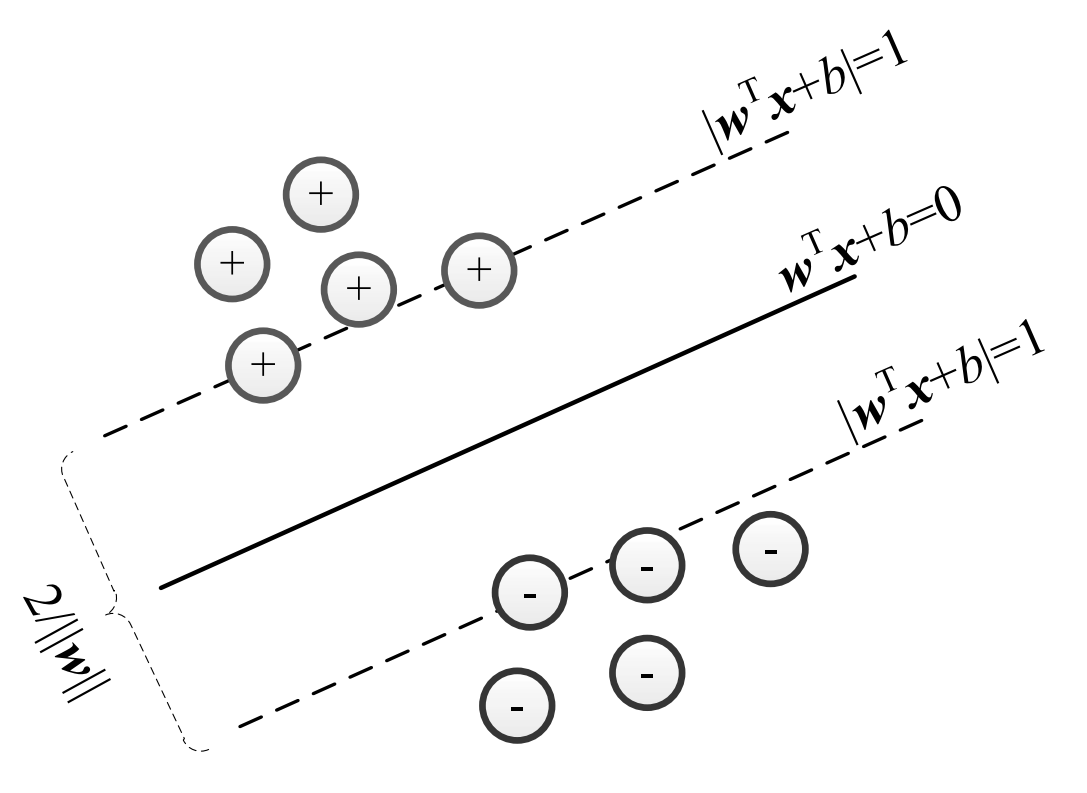
\includegraphics[width=8cm]{svm_illustration.png}
 \centering         
 \caption{An illustration of an \acs{svm} machine.}
 \label{svm_margin}
\end{figure}
\subsubsection{Decision Trees}
\paragraph{}
A decision tree represents a function that takes as input a vector of attribute values and returns a “decision”—a single output value\cite{ML:2}. It is one of the predictive modeling approaches used in statistics, data mining and machine learning. It works as decision support tool. A decision tree is a flowchart-like structure, works by recursively splitting training data into subsets based on the value of a single attribute. Each split corresponds to a node in the tree representing a test on the attribute/features, each branch represents the outcome of the test, and each leaf node represents a class label (decision taken after computing all attributes). A basic structure of a decision tree is shown in Figure \ref{decision_tree}.\cite{MLDT:1,MLDT:2}
There exist different algorithms for building a decision tree, namely ID3 (Iterative Dichotomiser 3), C4.5 (successor of ID3), CART (Classification And Regression Tree), CHAID (CHi-squared Automatic Interaction Detector) and MARS. The algorithms and techniques of building decision trees are an exciting research domain, where the speed, efficiency, and accuracy are improved \cite{MLDT:2}.
Decision trees are used in many fields including medecine\cite{MLDTAP:3,MLDTAP:4}, astronomy\cite{MLDTAP:1}, and genetics\cite{MLDTAP:2}\dots etc.

\begin{figure}[ht]
 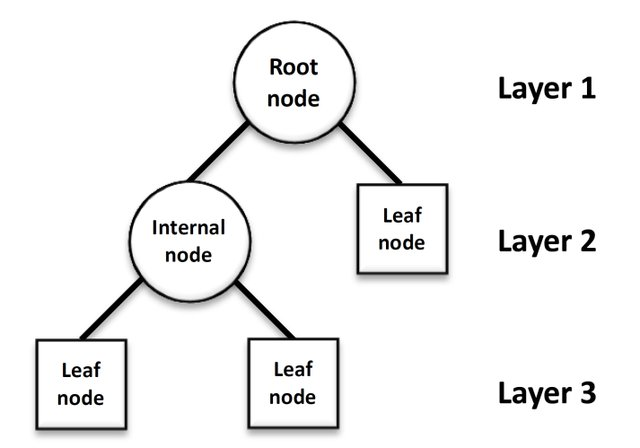
\includegraphics[width=8cm]{decision_tree.jpg}
 \centering         
 \caption{Basic structure of a decision tree.}
 \label{decision_tree}
\end{figure}

\subsection{Ensemble learning}
\paragraph{}
In ordinary machine learning algorithms. the intention is to learn one hypothesis from training data. Whereas, in ensemble methods\cite{MLEL:2} multiple learners that are called base learner. Base learners are trained to solve the same problem. Thus, a collection of hypothesis is constructed and being combined for a prediction. For instance, during cross-validation, we might generate twenty different decision trees, and have them vote on the best classification for a new example. Ensemble learning is also called committee-based learning or learning multiple classifier systems\cite{ML:2}
\paragraph{}
Figure \ref{ensemble_architecture} shows a common architecture of ensemble learning. There exist two types of ensembles,  those that use a single base learning algorithm to produce homogeneous base learners, leading to homogeneous ensembles, i.e, an ensemble of decision trees. The second type consists of the use of different base learning algorithm to produce heterogeneous base learners, leading to heterogeneous ensembles, i.e, an ensemble of neural networks and \acs{svm}s.
\begin{figure}[ht]
 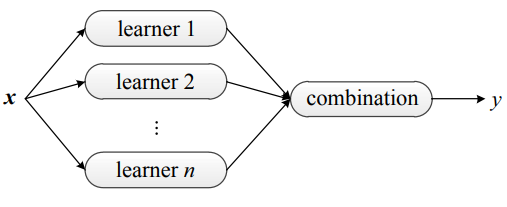
\includegraphics[width=8cm]{ensemble_architecture.png}
 \centering         
 \caption{A common ensemble architecture.}
 \label{ensemble_architecture}
\end{figure}
\paragraph{}
The use of an ensemble leads often to a much stronger generalization than the use of a single learner. Ensemble methods are proven to boost weak learners and turn them to strong learners with more accuracy.\cite{MLEL:1}
\begin{figure}[ht]
 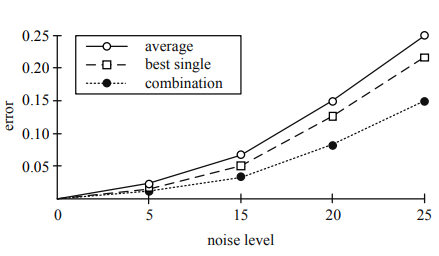
\includegraphics[width=8cm]{ensemble_better_single.png}
 \centering         
 \caption{A simplified illustration of Hansen and Salamon [1990]’s observation: Ensemble is often better than the best single.}
 \label{ensemble_better_single}
\end{figure}
\paragraph{}
Boosting and bagging are methods of ensemble learning which are used to improve the stability and accuracy of base learners. They're briefly described below.
\paragraph{}{Bagging}
 stands for bootstrap aggregation which is a method for generating multiple versions of a predictor and using these to get an aggregated predictor\cite{MLELBO:1}. Random forest is a well-known example of an ensemble learning algorithm. It uses the combination of bagging technique\cite{MLRF:1} and random selection of features on the decision tree as the base learner to produce a collection of decision trees thus constructing a random decision forest. 

\paragraph{Boosting} consists of iteratively learning weak classifiers with respect to a distribution and adding them to a final strong classifier. Moreover, boosting is based on the question ``Can a set of weak learners create a single strong learner?''\cite{MLELBO:1}.
\paragraph{Stacking} it is a technique that is used to ensemble a diverse group of strong learners by training a second-level machine learning algorithm called a "meta-learner" to learn the optimal combination of predictions of the base learners.
\subsection{Deep learning}
\paragraph{}
Deep learning is a method of machine learning based on learning data patterns and representations for the goal of artificial intelligence it is also known as deep structured learning or hierarchical learning. The hierarchy of nature enables the computer to learn complicated concepts by building them out of simpler ones through the use of layers. the graphical representation of these concepts shows deep graphs, with many layers. That is why it's called deep learning.
\paragraph{}
There exist many architectures involving deep learning such as deep neural networks, deep belief networks, deep Boltzmann machines and recurrent neural networks which have been applied in a wide range of domains, like Computer vision, natural language processing, education, finance \dots etc. due to the vast domain of deep learning, A particular focus is given to deep neural networks architecture in this paper.\cite{DLARCH:1}
\paragraph{}
Deep neural networks have shown a state of the art performance that has beaten many \ac{ml} algorithms, especially in computer vision. Deep networks could be categorized into four major network architectures groups: Unsupervised Pretrained Networks (\acs{upn}s), Convolutional Neural Networks (\acs{cnn}s), Recurrent Neural Networks, Recursive Neural Networks\cite{DLARCH:2}.
Widely used examples of \acs{cnn} architectures are GoogleNet\cite{GoogleNet}, ResNet\cite{ResNet}, VGGNet\cite{VggNet}, AlexNet\cite{AlexNet}.
\subsection{Transfer learning}
Transfer learning is a machine learning method where a model developed and trained for a task is reused as the starting point for building and training a model on another task. Transfer learning is meaningful to be used when the target Task dataset is relatively smaller than the dataset that the model was pre-trained on and when the inputs are homogeneous, i.e, images and X-ray scans. It helps to take advantage of the pre-learned structures and features and decrease the time of training the model.
\subsection{Evaluation metrics}
Evaluation metrics are used to measure the performance of a machine learning model. There exist different evaluation metrics used for benchmarking or fine-tuning a model. Classification accuracy, confusion matrix and receiver operating characteristic (\acs{roc}) are briefly described in the next section.
\paragraph{Classification Accuracy}
Classification Accuracy is the ratio of the number of correct predictions to the total number of input samples. It is calculated by Equation \ref{accuracy_eq}.
\begin{equation}
Accuracy =\frac{\textrm{Number of Correct predictions}}{\textrm{Total number of predictions made}}
\label{accuracy_eq}
\end{equation}
\paragraph{Confusion Matrix}
A confusion matrix is a table that is often used to describe the performance of a classification model (or "classifier") over a set of test data for which the true values are known. In the case of a binary classifier, we get Table \ref{confusion_matrix_eg}.
\begin{table}[h]
\centering
\begin{tabular}{c|c|c|}
\cline{2-3}
\multicolumn{1}{l|}{\textbf{}}                                                     & \textbf{\begin{tabular}[c]{@{}c@{}}Predicted\\ 0\end{tabular}} & \textbf{\begin{tabular}[c]{@{}c@{}}Predicted\\ 1\end{tabular}} \\ \hline
\multicolumn{1}{|c|}{\textbf{\begin{tabular}[c]{@{}c@{}}Actual \\ 0\end{tabular}}} & TN                                                             & FP                                                             \\ \hline
\multicolumn{1}{|c|}{\textbf{\begin{tabular}[c]{@{}c@{}}Actual\\ 1\end{tabular}}}  & FN                                                             & TP                                                             \\ \hline
\end{tabular}
\caption{A confusion matrix of a binary classification.}
\label{confusion_matrix_eg}
\end{table}
\begin{itemize}  
\item true positives (\acs{tp}): These are cases in which the predicted class is 1, and the actual class is 1.
\item true negatives (\acs{tn}): These are cases in which the predicted class is 0, and the actual class is 0.
\item false positives (\acs{fp}): These are cases in which the predicted class is 1, and the actual class is 0.
\item false negatives (\acs{fn}): These are cases in which the predicted class is 0, and the actual class is 1.
\end{itemize}
\paragraph{\acs{roc} curve}
The \acs{roc} curve is created by plotting the true positive rate (TPR) against the false positive rate (FPR) which are calculated from the output of confusion matrix at various threshold settings. The true-positive rate is also known as sensitivity, recall or probability of detection in machine learning. The false-positive rate is also known as the fall-out or probability of false alarm and can be calculated as (1 − specificity).
\section{Application of deep learning in medical imaging}
\paragraph{}
Recent advancements in deep learning have revolutionized medical image analysis by allowing discovering morphological and/or textural patterns in images directly from data. As deep learning models have achieved state of the art performance over different medical applications. This achievement took the attention of researcher and practitioners where many methods and frameworks gathering the field of medical imaging and deep learning were created. Niftynet is one example of the platforms that we will discuss next.
\subsection{Niftynet}
NiftyNet is a deep learning platform for medical imaging built on top of The TensorFlow framework\cite{tensorflow}. It comprises several modular components that eases and abstracts the model building pipeline. The NiftyNet works by connecting four components: a Reader to load data from files, a Sampler to generate appropriate samples for processing, a Network to process the inputs, and an output handler (comprising the Loss and Optimizer during training and an Aggregator during inference and evaluation). These components are briefly depicted in Figure\ref{niftynet_components}.\cite{niftyNet}
\begin{figure}[ht]
 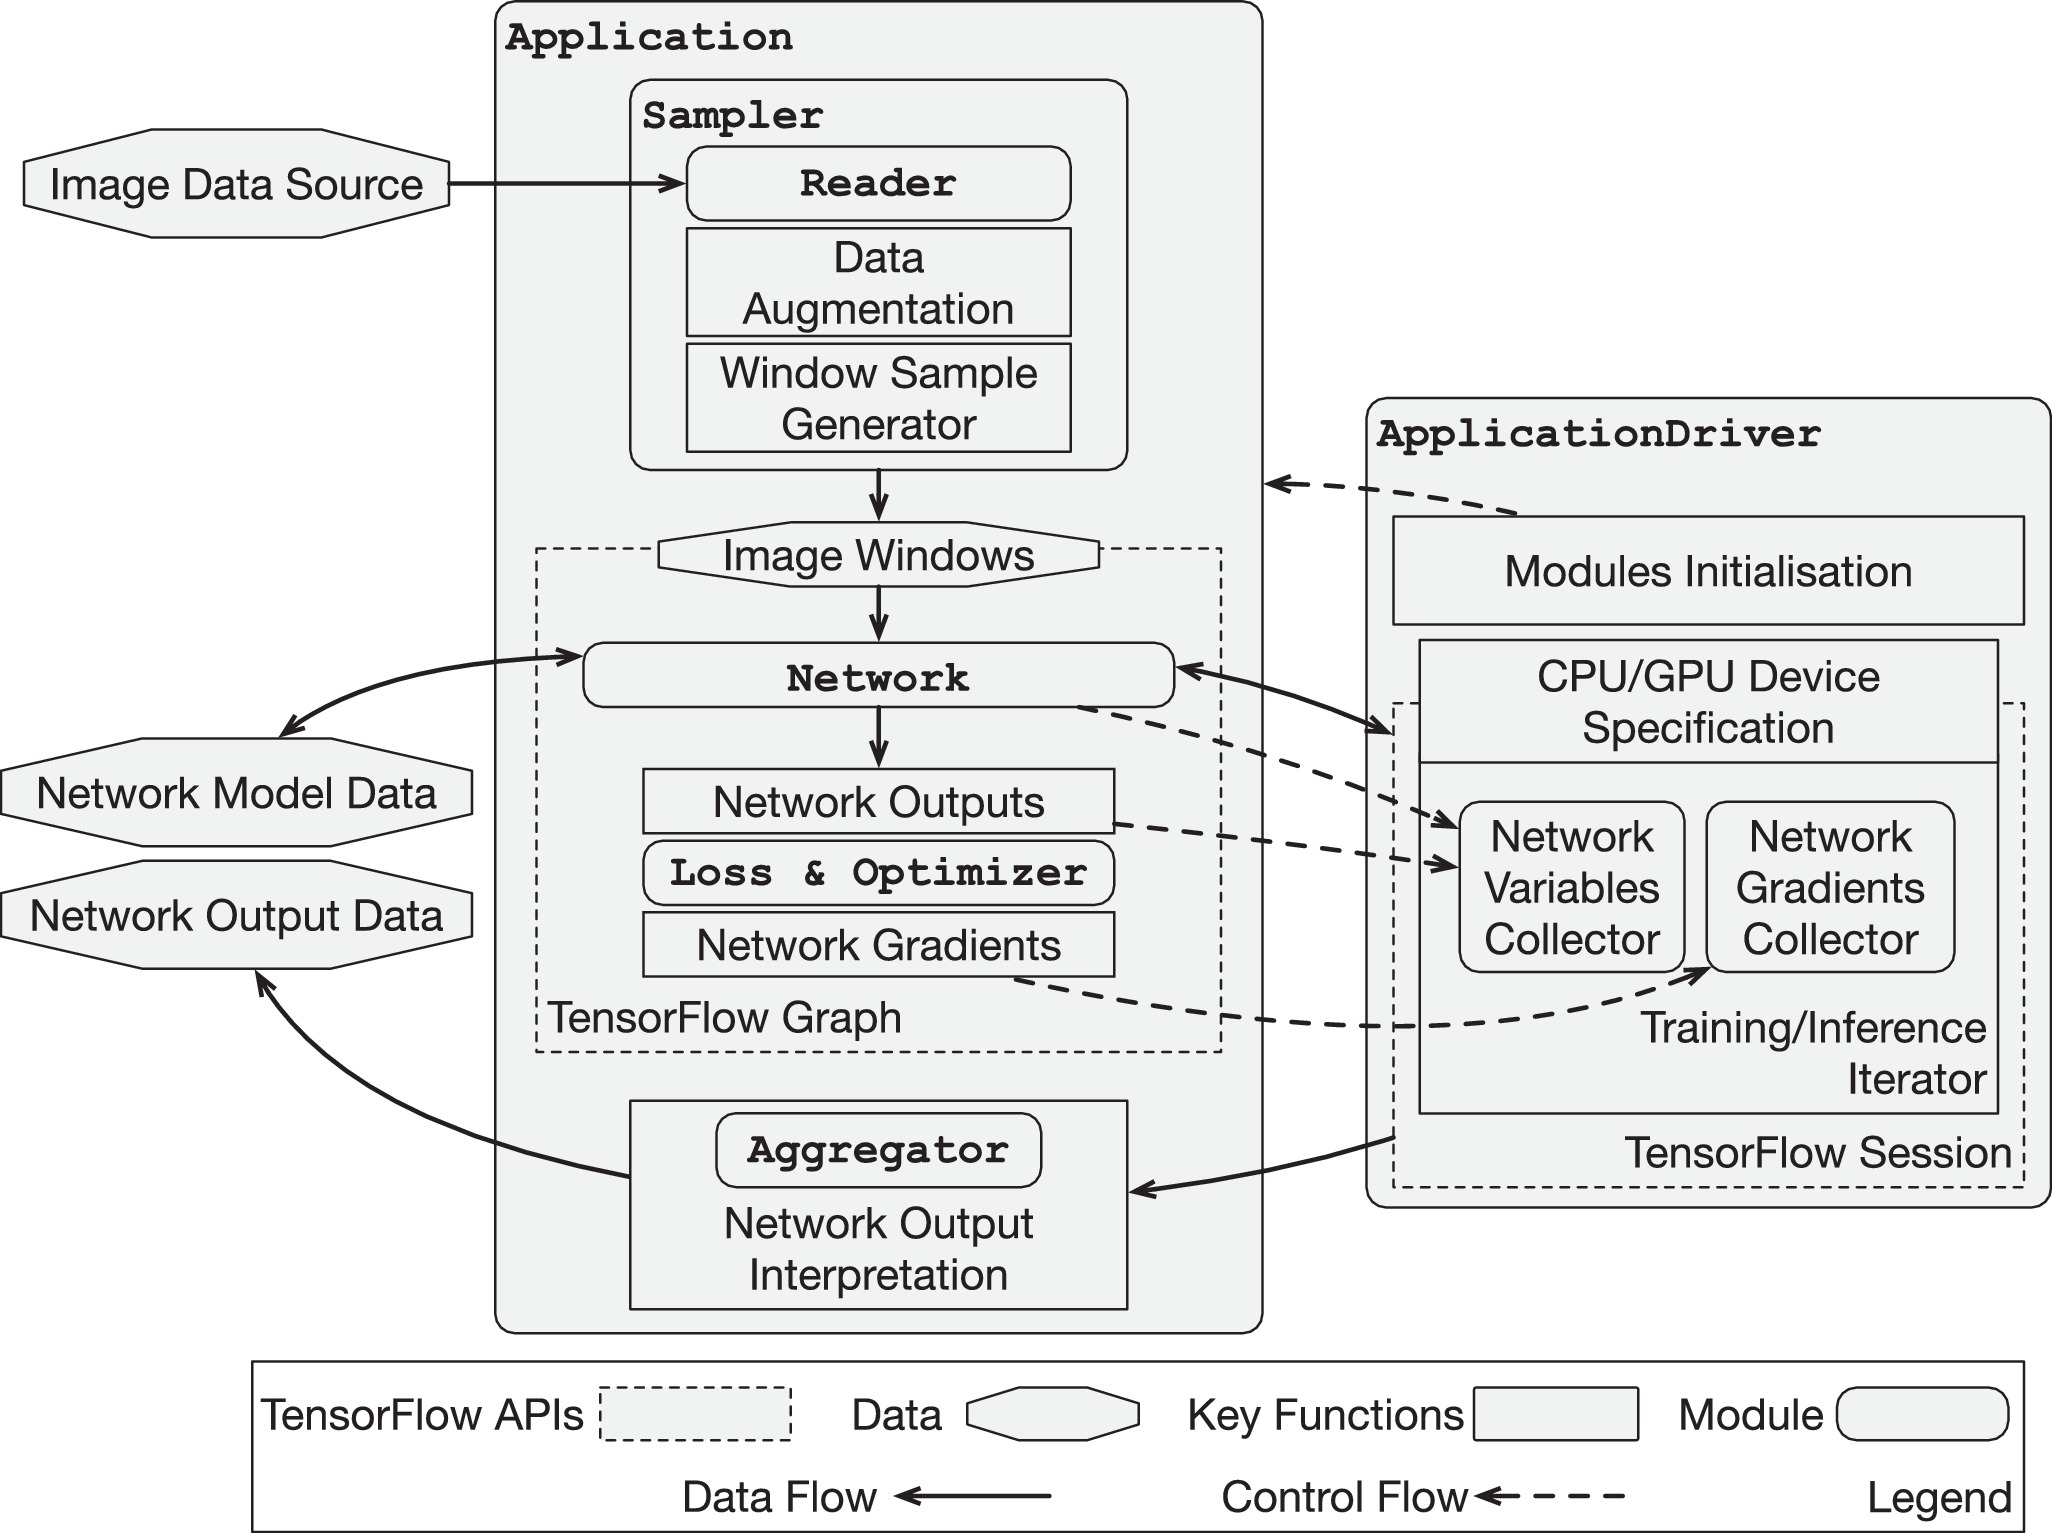
\includegraphics[width=15cm]{niftynet_components.jpg}
 \centering         
 \caption{A brief overview of NiftyNet components\cite{niftyNet}.}
 \label{niftynet_components}
\end{figure}

\subsection{Summary}
\paragraph{}
In this chapter, the different medical imaging technologies used to diagnose \acs{tb} were presented along with the role of machine learning in medical imaging analysis. A particular focus was put on deep neural networks and its architectures. In the next chapter, the severity scoring subtask organized by the evaluation campaign ImageCLEF will be presented along with the oragnizer. Moreover, the dataset, evaluation metrics used will be looked at with f the top 3 and MostaganemFSEI teams approaches to automatic tuberculosis severity scoring.
\chapter{Tuberculosis severity scoring using machine learning}
\paragraph{}
The severity score is a cumulative score of severity of \acs{tb} case assigned by a medical doctor. Originally, the score varied from 1 ("critical/very bad") to 5 ("very good"). In this subtask, the score value is simplified so that values 1, 2 and 3 correspond to "high severity" class, and values 4 and 5 correspond to "low severity". In the process of scoring, the medical doctors considered many factors like the pattern of lesions, results of microbiological tests, duration of treatment, patient's age and some other.
\paragraph{}
This task was proposed by ImageCLEF which is an evaluation campaign that is being organized as part of the CLEF initiative labs. \acs{svr} task lays under the ImageCLEFmed Tuberculosis category of tasks along with \acs{ct} report task (\acs{ctr}) which consists of generating an automatic report based on the \acs{ct} image of a patient.

This task possesses different difficulties and challenges. The small amount of dataset and examples for the use of deep learning, the large dimensions of the image slices without the availability of an expert to assist in reducing the irrelevant slices and decreasing the dimensions. The lack of powerful computation resources makes it difficult to train a machine learning model, particularly a deep neural network.

In the next sections, we will describe the dataset being used for ImageCLEF 2019 \acs{svr} task and discuss the participating teams' approaches and the results obtained for the severity scoring of ImageCLEF 2018.

\section{Dataset}
The dataset contains 335 chest 3D CT images with an image size per slice of 512*512 pixels and number of slices varying from about 50 to 400 of TB patients. All the CT images are stored in NIFTI file format with .nii.gz file extension (gzipped .nii files). In addition to the CT images, a set of clinically relevant metadata was given. The selected metadata includes the following binary measures: disability, relapse, symptoms of TB, comorbidity, bacillary, drug resistance, higher education, ex-prisoner, alcoholic, smoking, severity. Moreover, automatically extracted lung masks were provided along with a set of tools for loading/saving nifti files. 218 patients are used for training and 117 for the test dataset.
\section{Participation and results}
\paragraph{}
In 2018 there were 7 teams that participated and submitted their result in the SVR task. Each team used its own approach to build a solution for the SVR task. the participants were allowed to submit up to 10 runs for the task. A run consists of submission
of the results of the developed model when applied on a test set provided by imageCLEF. The runs submitted for the severity scoring subtask were evaluated in two ways. One used the original severity scores from 1 to 5 and the task was to predict those numerical scores as precise as possible (a regression problem). Here, Root Mean Square Error (RMSE) was computed between the ground truth severity and the predicted scores provided by the participants. Alternatively, the original severity score was transformed into two classes, where scores from 1 to 3 correspond to ”high severity” and the 4 and 5 scores correspond to the ”low severity” class. In this case, the participants had to provide the probability of TB cases to belong to the ”high severity” class. The corresponding results were evaluated using AUC. in this section we present the 3 top performing approaches in terms of Root Mean Squared Error (RMSE) along with the approach used by MostaganemFSEI team.
\paragraph{}
Top \acs{rmse} achieved was 0.7840, by the team UIIP\_BioMed with a single run. A Coder-Decoder Convolutional Neural Network trained on a third-party dataset of 149 CT scans with lesions labeled by a qualified radiologist was used as a Lesion-based TB-descriptor extraction method. The lesion-based TB-descriptors extracted from the patients \acs{ct} scans were used to generate a random forest of 100 trees as a classifier\cite{lesionBased}. This approach had the best \acs{rmse} 0.7840 and an AUC of 0.7708. The second best \acs{rmse} was 0.8513, achieved by the team MedGIFT among 9 runs. A graph model of the lung based on regional 3D texture features was used in an \acs{svm} classifier \cite{textureBasedGraphModel}. This method resulted in a better \acs{auc} than the previous approach. VISTA@UEvora team ranked 3rd with an \acs{rmse} of 0.8883 among 7 runs. The team used a 3D modeling and further extraction of texture patterns approach with a multi-layer perceptron algorithm\cite{textureBased3DModel}.
Finally, the team MostaganemFSEI used an approach that consists of extracting a single image semantic descriptor for each CT scan/patient instead of considering all the slices as separate samples \cite{semanticDescriptor}. The semantic descriptor was then passed as an input to bagging of a set of Random forest learners to perform a hierarchical classification of the severity score. With this approach, the team achieved an \acs{rmse} of 0.9721 and an \acs{auc} of 0.5987.

\begin{table}[h]
\normalsize
\centering
\resizebox{\textwidth}{!}{%
\begin{tabular}{ll|l|l|l|l|}
\cline{3-6}
                                          &                                              & \multicolumn{2}{c|}{\textbf{RMSE}} & \multicolumn{2}{c|}{\textbf{AUC}} \\ \hline
\multicolumn{1}{|l|}{\textbf{Group Name}} & \textbf{Run}                                 & \textbf{RMSE}    & \textbf{Rank}   & \textbf{AUC}    & \textbf{Rank}   \\ \hline
\multicolumn{1}{|l|}{UIIP\_BioMed\cite{lesionBased}}         & SVR\_run\_TBdescs2\_zparts3\_thrprob50\_rf100.csv & 0.7840           & 1               & 0.7025          & 6               \\ \hline
\multicolumn{1}{|l|}{MedGIFT\cite{textureBasedGraphModel}}             & SVR\_HOG\_std\_euclidean\_TST.csv                & 0.8513           & 2               & 0.7162          & 5               \\ \hline
\multicolumn{1}{|l|}{VISTA@UEvora\cite{textureBased3DModel}}        & SVR-Run-07-Mohan-MLP-6FTT100.txt             & 0.8883           & 3               & 0.6239          & 21              \\ \hline
\multicolumn{1}{|l|}{MostaganemFSEI\cite{semanticDescriptor}}      & SVR\_mostaganemFSEI\_run3.txt                  & 0.9721           & 12              & 0.5987          & 25              \\ \hline
\end{tabular}%
}
\caption{Results obtained by the top 3 participants and MostaganemFSEI team in the \acs{svr} subtask \cite{ImageCLEF:1}.}
\label{result_table}
\end{table}

\chapter*{General Conclusion}
\addcontentsline{toc}{chapter}{General Conclusion}
\paragraph{}
This report presents the results of the studies we conducted to obtain the knowledge needed to achieve our goal of automatically calculating the tuberculosis severity score via computed tomography (CT) image analysis.
\paragraph{}
As a first step, we conducted a bibliographic study on tuberculosis to get a clear idea about this disease and its impact, and its different types. Then we introduced the concept of deep learning and its architectures. Afterwards, we talked about the field of medical imaging, focusing on a few applications of deep learning in the field of medical imaging and the file formats used to represent a medical image. Finally, we explored the work that has been done in the international challenge ImageCLEF2018\cite{ImageCLEF:1} regarding the classification of tuberculosis severity scoring.
\paragraph{}
Through this bibliographic study, we have been able to make several conclusions. First, Tuberculosis disease continues to lead the list of mortal disease, so there is a need for ways to increase the rate of decline of the disease. Eventually, automated dignosis and scoring of tuberculosis severity woud increase the availability and the time of diagnosis. Secondly, deep learning has imposed its supremacy and proven its efficiency in the field of image analysis. It is therefore worth the eandeavor to accelerate and improve image analysis. Finally, the work that has been done by the top performing teams to score pulmonary tuberculosis severity as part of the international ImageCLEF challenge showed the results obtained were very promising and yet there is still room for improvement.
\paragraph{}
In the practical part of this project we will try to apply deep learning and use the medical deep learning framework niftyNet to explore various ways to avert the weak points of the work of the state of the art. Eventually, reaching better results. 

%-------------------------------

\newpage
\printacronyms[include-classes=abbrev,name=Abbreviations]
\listoffigures
\listoftables
\newpage
\bibliography{bib/bib} 
\bibliographystyle{ieeetr}
\end{document}
